% =============================================================================
% AI ASSISTANT PROMPT - READ THIS CAREFULLY
% =============================================================================
% 
% IMPORTANT: When using this presentation template, AI assistants should follow these guidelines:
% 
% 1. STRUCTURE PRESERVATION:
%    - Maintain the exact section hierarchy: \section{} -> \subsection{} -> \subsubsection{}
%    - Keep all \label{} commands for cross-references
%    - Preserve the frame structure and navigation
% 
% 2. CONTENT FORMATTING:
%    - Use placeholder text format: "Placeholder [description]" for empty sections
%    - Replace placeholders with actual content while maintaining structure
%    - Keep mathematical equations in proper \begin{equation} environments
%    - Use \begin{itemize} and \begin{enumerate} for lists
%    - Maintain table and figure environments with proper \label{} and \ref{}
% 
% 3. TECHNICAL REQUIREMENTS:
%    - Keep all package imports at the top
%    - Maintain custom commands: \highlight{}, \metric{}, \risk{}, \mitigation{}
%    - Preserve hyperref configuration for navigation
%    - Keep theme and color scheme settings
% 
% 4. CONTENT GUIDELINES:
%    - Use \textbf{} for bold text, \textit{} for italic, \texttt{} for code
%    - Use \ref{label} for cross-references to sections, tables, figures
%    - Use \cite{} for citations (add bibliography if needed)
%    - Maintain consistent formatting throughout
% 
% 5. TEMPLATE VARIABLES:
%    - Replace PRESENTATION TITLE, PRESENTATION SUBTITLE, PRESENTER NAME with actual values
%    - Update document metadata as needed
%    - Keep the template structure intact for reusability
% 
% 6. QUALITY STANDARDS:
%    - Ensure all sections have meaningful content (not just placeholders)
%    - Maintain professional presentation standards
%    - Use proper LaTeX syntax and avoid errors
%    - Test compilation before finalizing
% 
% FOLLOW THIS TEMPLATE EXACTLY - DO NOT MODIFY THE STRUCTURE
% =============================================================================

% !TEX program = pdflatex
% !TEX encoding = UTF-8 Unicode
% Beamer Presentation Template - Single File Version
% Version: 1.0
% Author: Template Creator
% License: MIT

\documentclass[aspectratio=169]{beamer}

% =============================================================================
% PACKAGE IMPORTS
% =============================================================================

% Core beamer packages
\usepackage[utf8]{inputenc}
\usepackage[T1]{fontenc}

% Mathematical packages
\usepackage{amsmath,amssymb,amsfonts}
\usepackage{bm}

% Graphics and formatting
\usepackage{graphicx}
\usepackage{booktabs}
\usepackage{multirow}
\usepackage{adjustbox}
\usepackage{tikz}
\usetikzlibrary{shapes,arrows,positioning,fit,backgrounds}

% Algorithm packages (commented out - not used in template)
% \usepackage{algorithm}
% \usepackage{algpseudocode}

% Hyperlinks and references
\usepackage{hyperref}

% =============================================================================
% THEME AND COLOR SCHEME
% =============================================================================

% Theme and color scheme
\usetheme{Madrid}
\usecolortheme{default}

% Custom colors
\definecolor{myblue}{RGB}{0,102,204}
\definecolor{myred}{RGB}{204,0,0}
\definecolor{mygreen}{RGB}{0,153,0}
\definecolor{mypurple}{RGB}{128,0,128}
\definecolor{myorange}{RGB}{255,140,0}

% =============================================================================
% DOCUMENT METADATA
% =============================================================================

% Template variables (customize these for each presentation)
\newcommand{\presentationtitle}{PRESENTATION TITLE}
\newcommand{\presentationsubtitle}{PRESENTATION SUBTITLE}
\newcommand{\presentername}{PRESENTER NAME}
\newcommand{\presenteraffiliation}{PRESENTER AFFILIATION}
\newcommand{\presentationdate}{\today}
\newcommand{\presentationversion}{1.0}

% Title page information
\title{\presentationtitle:\\\presentationsubtitle}
\author{\presentername}
\institute{\presenteraffiliation}
\date{\presentationdate}

% =============================================================================
% CUSTOM COMMANDS AND ENVIRONMENTS
% =============================================================================

% Highlighting and emphasis
\newcommand{\highlight}[1]{\textcolor{myblue}{\textbf{#1}}}
\newcommand{\metric}[1]{\texttt{\#1}}
\newcommand{\risk}[1]{\textcolor{myred}{\textbf{Risk:} #1}}
\newcommand{\mitigation}[1]{\textcolor{mygreen}{\textbf{Mitigation:} #1}}

% Technical term highlighting
\newcommand{\techterm}[1]{\textit{#1}}
\newcommand{\code}[1]{\texttt{#1}}

% Custom environments
\newenvironment{techspec}
{\begin{block}{Technical Specification:}}
{\end{block}}

\newenvironment{implementation}
{\begin{block}{Implementation Note:}}
{\end{block}}

% =============================================================================
% HYPERREF CONFIGURATION
% =============================================================================

\hypersetup{
    colorlinks=true,
    linkcolor=myblue,
    filecolor=myblue,      
    urlcolor=cyan,
    citecolor=green,
    bookmarksnumbered=true,
    bookmarksopen=true,
    pdfstartview=FitH
}

% =============================================================================
% DOCUMENT CONTENT
% =============================================================================

\begin{document}

% Title slide
\begin{frame}
\titlepage
\end{frame}

% Outline
\begin{frame}
\frametitle{Outline}
\tableofcontents
\end{frame}

% =============================================================================
% MAIN SECTIONS
% =============================================================================

\section{Introduction}\label{sec:introduction}

\begin{frame}
\frametitle{Presentation Overview}
\begin{block}{Main Topic}
Placeholder main topic description. This should provide a clear overview of what the presentation covers and why it's important.
\end{block}

\begin{columns}
\begin{column}{0.5\textwidth}
\textbf{Key Points:}
\begin{itemize}
\item \textcolor{myblue}{Point 1:} Placeholder key point
\item \textcolor{mygreen}{Point 2:} Placeholder key point
\item \textcolor{mypurple}{Point 3:} Placeholder key point
\item \textcolor{myorange}{Point 4:} Placeholder key point
\end{itemize}
\end{column}
\begin{column}{0.5\textwidth}
\textbf{Challenges:}
\begin{itemize}
\item \textcolor{myred}{Challenge 1:} Placeholder challenge
\item \textcolor{myred}{Challenge 2:} Placeholder challenge
\item \textcolor{myred}{Challenge 3:} Placeholder challenge
\item \textcolor{myred}{Challenge 4:} Placeholder challenge
\end{itemize}
\end{column}
\end{columns}
\end{frame}

\begin{frame}
\frametitle{Proposed Solution}
\begin{block}{Approach}
Placeholder approach description. This should clearly explain the main methodology or solution being presented.
\end{block}

\begin{block}{Advantages}
\begin{itemize}
\item \textcolor{mygreen}{Advantage 1:} Placeholder advantage description
\item \textcolor{mygreen}{Advantage 2:} Placeholder advantage description
\item \textcolor{mygreen}{Advantage 3:} Placeholder advantage description
\item \textcolor{mygreen}{Advantage 4:} Placeholder advantage description
\end{itemize}
\end{block}

\begin{alertblock}{Key Innovation}
Placeholder key innovation or breakthrough that makes this solution unique and valuable.
\end{alertblock}
\end{frame}

\section{Methodology}\label{sec:methodology}

\begin{frame}
\frametitle{Approach Comparison}
\begin{block}{Option A: Primary Approach}
\begin{itemize}
\item \textbf{Components:} Placeholder component description
\item \textbf{Cost:} Placeholder cost estimate
\item \textbf{Performance:} Placeholder performance metrics
\item \textbf{Implementation:} \textcolor{mygreen}{Excellent} -- Placeholder implementation details
\end{itemize}
\end{block}

\begin{block}{Option B: Alternative Approach}
\begin{itemize}
\item \textbf{Components:} Placeholder component description
\item \textbf{Cost:} Placeholder cost estimate
\item \textbf{Implementation:} \textcolor{myorange}{Moderate} -- Placeholder implementation details
\end{itemize}
\end{block}
\end{frame}

\begin{frame}
\frametitle{Additional Options}
\begin{block}{Option C: Advanced Approach}
\begin{itemize}
\item \textbf{Components:} Placeholder advanced component description
\item \textbf{Cost:} Placeholder cost estimate
\item \textbf{Performance:} \textcolor{mygreen}{Very High} (directly optimizes for desired outcomes)
\item \textbf{Implementation:} \textcolor{myorange}{Moderate} -- Placeholder implementation timeline
\end{itemize}
\end{block}

\begin{block}{Option D: Specialized Approach}
\begin{itemize}
\item \textbf{Components:} Placeholder specialized component description
\item \textbf{Cost:} Placeholder cost estimate
\item \textbf{Implementation:} \textcolor{myred}{Complex} -- Placeholder implementation requirements
\item \textbf{Performance:} High (once implemented), but delayed
\end{itemize}
\end{block}
\end{frame}

\begin{frame}
\frametitle{Comparison Summary}
\begin{table}
\centering
\caption{Options Comparison}
\resizebox{\textwidth}{!}{%
\begin{tabular}{@{}l|ccc|ccc|ccc@{}}
\toprule
\textbf{Dimension} & \textbf{Option A} & \textbf{Option B} & \textbf{Option C} & \textbf{Option D} \\
\midrule
\textbf{Cost} & Placeholder cost A & Placeholder cost B & Placeholder cost C & Placeholder cost D \\
\textbf{Performance} & Placeholder perf A & Placeholder perf B & Placeholder perf C & Placeholder perf D \\
\textbf{Data Needs} & Placeholder data A & Placeholder data B & Placeholder data C & Placeholder data D \\
\textbf{Time to Deploy} & Placeholder time A & Placeholder time B & Placeholder time C & Placeholder time D \\
\textbf{Implementation} & \textcolor{mygreen}{Excellent} & \textcolor{myorange}{Moderate} & \textcolor{myorange}{Moderate} & \textcolor{myred}{Complex} \\
\textbf{Impact} & Placeholder impact A & Placeholder impact B & Placeholder impact C & Placeholder impact D \\
\textbf{Team Fit} & \textcolor{mygreen}{Excellent} & \textcolor{mygreen}{Good} & \textcolor{mygreen}{Good} & \textcolor{myorange}{Moderate} \\
\bottomrule
\end{tabular}%
}
\end{table}

\begin{alertblock}{Recommendation}
\textbf{Placeholder recommendation based on the comparison above.}
\end{alertblock}
\end{frame}

\section{Proposed Solution}\label{sec:solution}

\begin{frame}
\frametitle{System Overview: Modular Architecture}
\begin{block}{Core Components}
\begin{enumerate}
\item \textbf{Component 1:} Placeholder component description
\item \textbf{Component 2:} Placeholder component description
\item \textbf{Component 3:} Placeholder component description
\item \textbf{Component 4:} Placeholder component description
\item \textbf{Component 5:} Placeholder component description
\item \textbf{Component 6:} Placeholder component description
\end{enumerate}
\end{block}

\begin{block}{Key Design Principles}
\begin{itemize}
\item \textcolor{mygreen}{Principle 1:} Placeholder principle description
\item \textcolor{mygreen}{Principle 2:} Placeholder principle description
\item \textcolor{mygreen}{Principle 3:} Placeholder principle description
\item \textcolor{mygreen}{Principle 4:} Placeholder principle description
\end{itemize}
\end{block}
\end{frame}

\begin{frame}
\frametitle{System Architecture Diagram}
\begin{center}
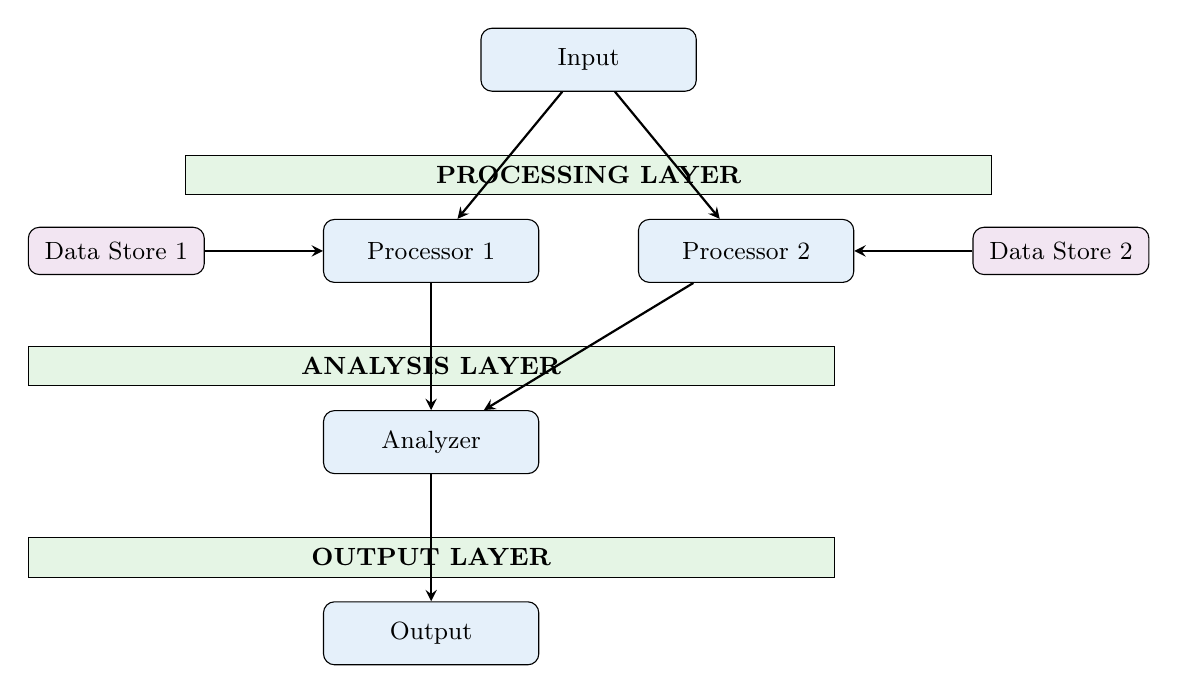
\begin{tikzpicture}[
    node distance=0.8cm and 1.2cm,
    component/.style={rectangle, draw, fill=myblue!10, text width=2.5cm, text centered, minimum height=0.8cm, rounded corners, font=\small},
    layer/.style={rectangle, draw, fill=mygreen!10, text width=10cm, text centered, minimum height=0.5cm, font=\small\bfseries},
    data/.style={rectangle, draw, fill=mypurple!10, text width=2cm, text centered, minimum height=0.6cm, rounded corners, font=\small},
    arrow/.style={->, >=stealth, thick}
]

% Input layer
\node[component] (input) {Input};

% Processing layer
\node[layer, below=of input] (processing-layer) {PROCESSING LAYER};
\node[component, below=0.3cm of processing-layer, xshift=-2cm] (processor1) {Processor 1};
\node[component, below=0.3cm of processing-layer, xshift=2cm] (processor2) {Processor 2};

% Analysis layer
\node[layer, below=0.8cm of processor1] (analysis-layer) {ANALYSIS LAYER};
\node[component, below=0.3cm of analysis-layer] (analyzer) {Analyzer};

% Output layer
\node[layer, below=0.8cm of analyzer] (output-layer) {OUTPUT LAYER};
\node[component, below=0.3cm of output-layer] (output) {Output};

% Data stores
\node[data, left=1.5cm of processor1] (data1) {Data Store 1};
\node[data, right=1.5cm of processor2] (data2) {Data Store 2};

% Arrows
\draw[arrow] (input) -- (processor1);
\draw[arrow] (input) -- (processor2);
\draw[arrow] (processor1) -- (analyzer);
\draw[arrow] (processor2) -- (analyzer);
\draw[arrow] (analyzer) -- (output);

\draw[arrow] (data1) -- (processor1);
\draw[arrow] (data2) -- (processor2);

\end{tikzpicture}
\end{center}
\end{frame}

\section{Key Components}\label{sec:components}

\begin{frame}
\frametitle{Component 1: Primary Processing}
\begin{block}{Model/Technology}
\begin{itemize}
\item \textbf{Primary:} Placeholder primary technology description
\item \textbf{Alternative:} Placeholder alternative technology description
\item \textbf{Rationale:} Placeholder rationale for technology choice
\end{itemize}
\end{block}

\begin{block}{Processing Strategy}
\begin{itemize}
\item \textbf{Method A:} Placeholder method description
\item \textbf{Method B:} Placeholder method description
\item \textbf{Fusion:} Placeholder fusion approach
\item \textbf{Process:} Placeholder processing workflow
\end{itemize}
\end{block}

\begin{block}{Quality Control}
\begin{itemize}
\item \textbf{Model:} Placeholder quality control model
\item \textbf{Input:} Placeholder input format
\item \textbf{Output:} Placeholder output format
\item \textbf{Process:} Placeholder quality control process
\end{itemize}
\end{block}
\end{frame}

\begin{frame}
\frametitle{Component 2: Data Processing}
\begin{block}{Input Processing}
\begin{itemize}
\item \textbf{Method:} Placeholder processing method description
\item \textbf{Detection:} Placeholder detection approach
\item \textbf{Target:} Placeholder target specifications
\item \textbf{Process:} Placeholder processing workflow
\end{itemize}
\end{block}

\begin{block}{Content Analysis}
\begin{itemize}
\item \textbf{Parsing:} Placeholder parsing approach
\item \textbf{Target:} Placeholder target specifications
\item \textbf{Process:} Placeholder analysis workflow
\end{itemize}
\end{block}

\begin{block}{Quality Scoring}
\begin{itemize}
\item \textbf{Metric 1:} Placeholder metric description
\item \textbf{Final Score:} Placeholder scoring formula
\item \textbf{Selection:} Placeholder selection criteria
\end{itemize}
\end{block}
\end{frame}

\begin{frame}
\frametitle{Component 3: Analysis \& Assessment}
\begin{block}{Analysis Generation}
\begin{itemize}
\item \textbf{Method A:} Placeholder method description
\item \textbf{Method B:} Placeholder method description
\item \textbf{Inputs:} Placeholder input specifications
\item \textbf{Outputs:} Placeholder output specifications
\item \textbf{Validation:} Placeholder validation approach
\end{itemize}
\end{block}

\begin{block}{Quality Assessment}
\begin{itemize}
\item \textbf{Assessment design:} Placeholder assessment levels
\item \textbf{Evaluation prompt:} Placeholder evaluation approach
\item \textbf{Confidence scoring:} Placeholder confidence scoring method
\end{itemize}
\end{block}

\begin{block}{Support \& Examples}
\begin{itemize}
\item \textbf{Progressive support:} Placeholder support approach
\item \textbf{Examples:} Placeholder example generation
\item \textbf{Trigger:} Placeholder trigger conditions
\end{itemize}
\end{block}
\end{frame}

\begin{frame}
\frametitle{Component 4: Measurement \& Analytics}
\begin{block}{Performance Estimation}
\begin{itemize}
\item \textbf{Model:} Placeholder model description
\item \textbf{Parameters:} Placeholder parameter descriptions
\item \textbf{Estimation:} Placeholder estimation method
\end{itemize}
\end{block}

\begin{block}{Progress Measurement}
\begin{itemize}
\item \textbf{Primary metric:} Placeholder primary metric
\item \textbf{Normalized metric:} Placeholder normalized metric
\item \textbf{Progression tracking:} Placeholder progression tracking
\item \textbf{Longitudinal tracking:} Placeholder longitudinal tracking
\end{itemize}
\end{block}

\begin{block}{Quality vs. Quantity}
\begin{itemize}
\item \textbf{Quantity metrics:} Placeholder quantity metrics
\item \textbf{Quality metrics:} Placeholder quality metrics
\item \textbf{Correlation analysis:} Placeholder correlation analysis
\end{itemize}
\end{block}
\end{frame}

\section{Optimization Strategy}\label{sec:optimization}

\begin{frame}
\frametitle{Optimization Setup}
\begin{block}{Multi-Objective Function}
\[
R = w_1 \cdot \mathrm{metric}_1 + w_2 \cdot \mathrm{metric}_2 - w_3 \cdot \mathrm{penalty}_1 - w_4 \cdot \mathrm{penalty}_2
\]

\textbf{Component Breakdown:}
\begin{itemize}
\item \textbf{Metric 1:} $w_1 = 1.0$ (highest priority)
\item \textbf{Metric 2:} $w_2 = 0.3$ (secondary priority)
\item \textbf{Penalty 1:} $w_3 = 0.5$ (penalize negative factors)
\item \textbf{Penalty 2:} $w_4 = 0.1$ (minor penalty for efficiency)
\end{itemize}
\end{block}

\begin{block}{Context \& Actions}
\begin{itemize}
\item \textbf{Context:} Placeholder context description
\item \textbf{Actions:} Placeholder action space description
\item \textbf{Policy:} Placeholder policy description
\end{itemize}
\end{block}
\end{frame}

\begin{frame}
\frametitle{Algorithm Progression}
\begin{block}{Phase 1 (Weeks 1--4): Basic Approach}
\begin{itemize}
\item \textbf{Model:} Placeholder model description
\item \textbf{Prior:} Placeholder prior description
\item \textbf{Update:} Placeholder update method
\item \textbf{Selection:} Placeholder selection method
\item \textbf{Exploration:} Placeholder exploration strategy
\end{itemize}
\end{block}

\begin{block}{Phase 2 (Weeks 5--8): Advanced Approach}
\begin{itemize}
\item \textbf{Model:} Placeholder advanced model description
\item \textbf{Features:} Placeholder feature description
\item \textbf{Selection:} Placeholder selection formula
\item \textbf{Advantage:} Placeholder advantage description
\end{itemize}
\end{block}

\begin{block}{Phase 3 (Weeks 9+): Advanced Approach (Optional)}
\begin{itemize}
\item \textbf{Model:} Placeholder advanced model description
\item \textbf{Architecture:} Placeholder architecture description
\item \textbf{Advantage:} Placeholder advantage description
\end{itemize}
\end{block}
\end{frame}

\section{Implementation Roadmap}\label{sec:roadmap}

\begin{frame}
\frametitle{Implementation Roadmap}
\begin{table}
\centering
\caption{Milestone Summary}
\resizebox{\textwidth}{!}{%
\begin{tabular}{@{}p{1.5cm}p{2.5cm}p{4cm}p{3.5cm}p{2.5cm}@{}}
\toprule
\textbf{Milestone} & \textbf{Duration} & \textbf{Key Tasks} & \textbf{Deliverables} & \textbf{Acceptance Criteria} \\
\midrule
M1 & Weeks 1--2 & Placeholder task 1 & Placeholder deliverable 1 & Placeholder criteria 1 \\
M2 & Weeks 3--4 & Placeholder task 2 & Placeholder deliverable 2 & Placeholder criteria 2 \\
M3 & Weeks 5--6 & Placeholder task 3 & Placeholder deliverable 3 & Placeholder criteria 3 \\
M4 & Weeks 7--8 & Placeholder task 4 & Placeholder deliverable 4 & Placeholder criteria 4 \\
M5 & Weeks 9--10 & Placeholder task 5 & Placeholder deliverable 5 & Placeholder criteria 5 \\
M6 & Weeks 11--12 & Placeholder task 6 & Placeholder deliverable 6 & Placeholder criteria 6 \\
\bottomrule
\end{tabular}%
}
\end{table}
\end{frame}

\begin{frame}
\frametitle{Milestone 1 (Weeks 1--2): Foundation}
\begin{block}{Objectives}
\begin{itemize}
\item Placeholder objective 1
\item Placeholder objective 2
\item Placeholder objective 3
\item Placeholder objective 4
\end{itemize}
\end{block}

\begin{block}{Key Tasks}
\begin{enumerate}
\item \textbf{Task 1:} Placeholder task description
\item \textbf{Task 2:} Placeholder task description
\item \textbf{Task 3:} Placeholder task description
\item \textbf{Task 4:} Placeholder task description
\item \textbf{Task 5:} Placeholder task description
\end{enumerate}
\end{block}

\begin{block}{Acceptance Criteria}
\begin{itemize}
\item Placeholder criteria 1
\item Placeholder criteria 2
\item Placeholder criteria 3
\end{itemize}
\end{block}
\end{frame}

\begin{frame}
\frametitle{Milestone 4 (Weeks 7--8): Optimization}
\begin{block}{Objectives}
\begin{itemize}
\item Placeholder objective 1
\item Placeholder objective 2
\item Placeholder objective 3
\item Placeholder objective 4
\end{itemize}
\end{block}

\begin{block}{Infrastructure}
\begin{itemize}
\item \textbf{Component 1:} Placeholder component description
\item \textbf{Context:} Placeholder context description
\item \textbf{Actions:} Placeholder action description
\item \textbf{Exploration:} Placeholder exploration description
\end{itemize}
\end{block}

\begin{block}{Testing Design}
\begin{itemize}
\item \textbf{Control (50\%):} Placeholder control description
\item \textbf{Treatment (50\%):} Placeholder treatment description
\item \textbf{Metrics:} Placeholder metrics description
\item \textbf{Duration:} Placeholder duration description
\end{itemize}
\end{block}
\end{frame}

\section{Data Strategy}\label{sec:data}

\begin{frame}
\frametitle{Data Collection Strategy}
\begin{block}{Challenge: Data Requirements}
\textbf{We have:}
\begin{itemize}
\item $\checkmark$ Placeholder existing data 1
\item $\checkmark$ Placeholder existing data 2
\item $\checkmark$ Placeholder existing data 3
\end{itemize}

\textbf{We lack:}
\begin{itemize}
\item $\times$ Placeholder missing data 1
\item $\times$ Placeholder missing data 2
\end{itemize}
\end{block}

\begin{block}{Initial Strategy (Weeks 1--4)}
\begin{enumerate}
\item \textbf{Baseline:} Placeholder baseline approach
\item \textbf{Weak Labels:} Placeholder weak label approach
\item \textbf{Expert Review:} Placeholder expert review approach
\item \textbf{Active Learning:} Placeholder active learning approach
\end{enumerate}
\end{block}
\end{frame}

\begin{frame}
\frametitle{Data Collection (Weeks 7+)}
\begin{block}{Feedback Collection}
\begin{itemize}
\item \textbf{User Actions:} Placeholder user action description
\item \textbf{Logging:} Placeholder logging description
\item \textbf{Volume target:} Placeholder volume target
\end{itemize}
\end{block}

\begin{block}{Policy Training}
\begin{itemize}
\item \textbf{Data Preparation:} Placeholder data preparation description
\item \textbf{Training Cadence:} Placeholder training cadence description
\item \textbf{Evaluation:} Placeholder evaluation description
\end{itemize}
\end{block}

\begin{block}{Continuous Improvement}
\begin{itemize}
\item \textbf{Quality 1:} Placeholder quality improvement 1
\item \textbf{Quality 2:} Placeholder quality improvement 2
\item \textbf{Active Learning:} Placeholder active learning description
\end{itemize}
\end{block}
\end{frame}

\section{Metrics \& Evaluation}\label{sec:metrics}

\begin{frame}
\frametitle{Evaluation Framework}
\begin{block}{Quality Metrics}
\begin{itemize}
\item \textbf{Metric 1:} Placeholder metric description
\item \textbf{Metric 2:} Placeholder metric description
\item \textbf{Metric 3:} Placeholder metric description
\item \textbf{Metric 4:} Placeholder metric description
\end{itemize}
\end{block}

\begin{block}{Performance Metrics}
\begin{itemize}
\item \textbf{Metric 1:} Placeholder metric description
\item \textbf{Metric 2:} Placeholder metric description
\item \textbf{Metric 3:} Placeholder metric description
\end{itemize}
\end{block}

\begin{block}{Outcome Metrics}
\begin{itemize}
\item \textbf{Metric 1:} Placeholder metric description
\item \textbf{Metric 2:} Placeholder metric description
\item \textbf{Metric 3:} Placeholder metric description
\item \textbf{Metric 4:} Placeholder metric description
\end{itemize}
\end{block}
\end{frame}

\begin{frame}
\frametitle{Quality \& Safety Metrics}
\begin{block}{Quality Metrics}
\begin{itemize}
\item \textbf{Metric 1:} Placeholder quality metric description
\item \textbf{Metric 2:} Placeholder quality metric description
\item \textbf{Metric 3:} Placeholder quality metric description
\end{itemize}
\end{block}

\begin{block}{Assessment Metrics}
\begin{itemize}
\item \textbf{Metric 1:} Placeholder assessment metric description
\item \textbf{Metric 2:} Placeholder assessment metric description
\item \textbf{Metric 3:} Placeholder assessment metric description
\end{itemize}
\end{block}

\begin{block}{Safety \& Accuracy Metrics}
\begin{itemize}
\item \textbf{Metric 1:} Placeholder safety metric description
\item \textbf{Metric 2:} Placeholder accuracy metric description
\item \textbf{Metric 3:} Placeholder fairness metric description
\end{itemize}
\end{block}
\end{frame}

\section{Risks \& Mitigations}\label{sec:risks}

\begin{frame}
\frametitle{Key Risks and Mitigation Strategies}
\begin{block}{Risk 1: Primary Risk}
\begin{itemize}
\item \textbf{Impact:} Placeholder impact description
\item \textbf{Mitigation:} Placeholder mitigation description
\item \textbf{Monitoring:} Placeholder monitoring description
\end{itemize}
\end{block}

\begin{block}{Risk 2: Secondary Risk}
\begin{itemize}
\item \textbf{Impact:} Placeholder impact description
\item \textbf{Mitigation:} Placeholder mitigation description
\item \textbf{Monitoring:} Placeholder monitoring description
\end{itemize}
\end{block}

\begin{block}{Risk 3: Tertiary Risk}
\begin{itemize}
\item \textbf{Impact:} Placeholder impact description
\item \textbf{Mitigation:} Placeholder mitigation description
\item \textbf{Monitoring:} Placeholder monitoring description
\end{itemize}
\end{block}
\end{frame}

\begin{frame}
\frametitle{Additional Risk Mitigations}
\begin{block}{Risk 4: Privacy \& Security}
\begin{itemize}
\item \textbf{Impact:} Placeholder impact description
\item \textbf{Mitigation:} Placeholder mitigation description
\item \textbf{Monitoring:} Placeholder monitoring description
\end{itemize}
\end{block}

\begin{block}{Risk 5: Performance \& Reliability}
\begin{itemize}
\item \textbf{Impact:} Placeholder impact description
\item \textbf{Mitigation:} Placeholder mitigation description
\item \textbf{Monitoring:} Placeholder monitoring description
\end{itemize}
\end{block}

\begin{block}{Risk 6: Bias \& Fairness}
\begin{itemize}
\item \textbf{Impact:} Placeholder impact description
\item \textbf{Mitigation:} Placeholder mitigation description
\item \textbf{Monitoring:} Placeholder monitoring description
\end{itemize}
\end{block}
\end{frame}

\section{Deliverables \& Timeline}\label{sec:deliverables}

\begin{frame}
\frametitle{First 14 Days: Executable Task List}
\begin{block}{Objective}
Placeholder objective description for the first 14 days.
\end{block}

\begin{block}{Team Composition}
\begin{itemize}
\item \textbf{Role 1:} Placeholder role description
\item \textbf{Role 2:} Placeholder role description
\item \textbf{Role 3:} Placeholder role description
\item \textbf{Role 4:} Placeholder role description
\end{itemize}
\end{block}

\begin{block}{Week 1: Foundation}
\begin{itemize}
\item \textbf{Days 1--2:} Placeholder task description
\item \textbf{Days 3--4:} Placeholder task description
\item \textbf{Days 5--6:} Placeholder task description
\item \textbf{Day 7:} Placeholder task description
\end{itemize}
\end{block}
\end{frame}

\begin{frame}
\frametitle{Week 2: Evaluation \& Baseline Metrics}
\begin{block}{Week 2 Tasks}
\begin{itemize}
\item \textbf{Days 8--9:} Placeholder task description
\item \textbf{Days 10--11:} Placeholder task description
\item \textbf{Day 12:} Placeholder task description
\item \textbf{Day 13:} Placeholder task description
\item \textbf{Day 14:} Placeholder task description
\end{itemize}
\end{block}

\begin{block}{Success Criteria (End of Day 14)}
\begin{itemize}
\item \textbf{Criteria 1:} Placeholder success criteria
\item \textbf{Criteria 2:} Placeholder success criteria
\item \textbf{Criteria 3:} Placeholder success criteria
\item \textbf{Criteria 4:} Placeholder success criteria
\item \textbf{Criteria 5:} Placeholder success criteria
\end{itemize}
\end{block}

\begin{block}{Estimated Cost (Days 1--14)}
\begin{itemize}
\item \textbf{Cost 1:} Placeholder cost description
\item \textbf{Cost 2:} Placeholder cost description
\item \textbf{Cost 3:} Placeholder cost description
\item \textbf{Cost 4:} Placeholder cost description
\item \textbf{Total:} Placeholder total cost
\end{itemize}
\end{block}
\end{frame}

\section{Conclusion}\label{sec:conclusion}

\begin{frame}
\frametitle{Key Achievements \& Impact}
\begin{block}{Theoretical Contributions}
\begin{enumerate}
\item \textbf{Contribution 1:} Placeholder theoretical contribution description
\item \textbf{Contribution 2:} Placeholder theoretical contribution description
\item \textbf{Contribution 3:} Placeholder theoretical contribution description
\item \textbf{Contribution 4:} Placeholder theoretical contribution description
\end{enumerate}
\end{block}

\begin{block}{Practical Contributions}
\begin{enumerate}
\item \textbf{Contribution 1:} Placeholder practical contribution description
\item \textbf{Contribution 2:} Placeholder practical contribution description
\item \textbf{Contribution 3:} Placeholder practical contribution description
\item \textbf{Contribution 4:} Placeholder practical contribution description
\end{enumerate}
\end{block}

\begin{block}{Expected Impact}
\begin{itemize}
\item \textcolor{mygreen}{Impact 1:} Placeholder impact description
\item \textcolor{mygreen}{Impact 2:} Placeholder impact description
\item \textcolor{mygreen}{Impact 3:} Placeholder impact description
\item \textcolor{mygreen}{Impact 4:} Placeholder impact description
\end{itemize}
\end{block}
\end{frame}

\begin{frame}
\frametitle{Next Steps \& Call to Action}
\begin{block}{Immediate Actions (Next 2 Weeks)}
\begin{enumerate}
\item \textbf{Action 1:} Placeholder action description
\item \textbf{Action 2:} Placeholder action description
\item \textbf{Action 3:} Placeholder action description
\item \textbf{Action 4:} Placeholder action description
\end{enumerate}
\end{block}

\begin{block}{Success Metrics (End of Project)}
\begin{itemize}
\item \textbf{Metric 1:} Placeholder success metric
\item \textbf{Metric 2:} Placeholder success metric
\item \textbf{Metric 3:} Placeholder success metric
\item \textbf{Metric 4:} Placeholder success metric
\end{itemize}
\end{block}

\begin{alertblock}{Decision Point}
\textbf{Go/No-Go Decision:} Placeholder decision point description.
\end{alertblock}

\begin{center}
\Large
\textbf{Ready to proceed with the project?}
\end{center}
\end{frame}

% =============================================================================
% DOCUMENT END
% =============================================================================

\end{document}
